\documentclass[punct]{ctexbeamer}
\usefonttheme{professionalfonts}   % 数学公式字体

\titlegraphic{
\includegraphics[width=2cm]{tjnu.jpg}}

\usepackage{color}
%\lineskip=9pt
\linespread{1.3}\selectfont
\makeatletter
\renewcommand\normalsize{%
    \@setfontsize\normalsize\@xpt\@xiipt
    \abovedisplayskip 3\p@ \@plus3\p@ \@minus3\p@
    \abovedisplayshortskip \z@ \@plus3\p@
    \belowdisplayshortskip 3\p@ \@plus3\p@ \@minus1\p@
    \belowdisplayskip \abovedisplayskip
    \let\@listi\@listI}
\makeatother
\parskip=6pt
%\usepackage{ctex}
%\usepackage[UTF8, heading = false, scheme = plain]{ctex}
%%%=== theme ===%%%
\usetheme{Madrid}
\useinnertheme{circles}
\setbeamertemplate{navigation symbols}{}
%\setbeamertemplate{footline}[page number]
\setbeamertemplate{footline}[frame number]{}
\usepackage{lmodern}
\usepackage{amsmath}
\usepackage{amssymb}
\usepackage{latexsym}
\usepackage{amsthm}
\usepackage{mathrsfs}
\usepackage{tikz}




\setbeamertemplate{theorems}[numbered]
\newtheorem{thm}{定理}[section]
\newtheorem{prop}[thm]{命题}
\newtheorem{cor}[thm]{推论}
\newtheorem{defi}[thm]{定义}
\newtheorem{lem}[thm]{引理}

\newtheorem{quest}[thm]{问题}
\newtheorem{conj}[thm]{猜想}
\newtheorem{ex}{例}[section]
\newtheorem{pr}{性质}

\definecolor{blue}{rgb}{0,0.08,1}
\newcommand{\blue}{\textcolor{blue}}
\def\pf{\noindent {\bf 证明\ }}
\def\sol{\noindent {\bf 解\ }}


\def\multiset#1#2{\ensuremath{\left(\kern-.3em\left(\genfrac{}{}{0pt}{}{#1}{#2}\right)\kern-.3em\right)}}

\begin{document}
	\title{组\ 合\ 数\ 学}

	\author{张\ 彪}
	\institute[数学科学学院]{\normalsize 天津师范大学}
	%\date[2011年10月13日]{\small 2011年10月13日}
	\date[]{zhang@tjnu.edu.cn}
	\frame[plain]{\titlepage}
	\begin{frame}{{第6章\quad 递推关系}}
		\tableofcontents
	\end{frame}
	\AtBeginSection[]
	{
		\begin{frame}
			\frametitle{递推关系}
			\tableofcontents[currentsection]
		\end{frame}
	}
\begin{frame}
\begin{itemize}
\item 	递推关系几乎在所有的数学分支中都有重要作用, 对于组合数学更是如此.

\item 这 是因为每个组合问题都有它的组合结构, 而在许多情况下递推关系是刻画组合结 构的最合适的工具.

\item 如何建立递推关系, 已给的递推关系有何性质, 以及如何求解 递推关系等, 是递推关系中的几个基本问题.


\item  本章首先讨论递推关系的建立问题, 然后对一些常见的递推关系做比较深人 的讨论, 并给出其解法.
\end{itemize}

	\end{frame}
\section{递推关系的建立}
\begin{frame}{递推关系的建立}
	在 4.3.2 小节中讨论集合 $\{1,2, \cdots, n\}$ 的错排数 $D_n$ 时, 我们建立了关于 $D_n$ 的 递推关系
	\[
	\left\{\begin{array}{l}
	D_n=(n-1)\left(D_{n-1}+D_{n-2}\right) \quad(n \geqslant 3), \\
	D_1=0, \quad D_2=1,
	\end{array}\right.\tag{6.1.1}
\]
	并由此推出了
	\[
	\left\{\begin{array}{l}
	D_n=n D_{n-1}+(-1)^n \quad(n \geqslant 2), \\
	D_1=0 .
	\end{array}\right.\tag{6.1.2}
	\]
	\begin{itemize}
	\item  等式 (6.1.1) 给出了 $n$ 元错排 数 $D_n$ 同 $n-1$ 元错排数及 $n-2$ 元错排数 $D_{n-2}$ 之间的关系, 这样, 由初值 $D_1$ 和 $D_2$ 就可以计算出 $D_3$, 由 $D_2$ 和 $D_3$ 又可以计算出 $D_4$, 如此可以逐个计算出错排数序列 $D_1, D_2, D_3, \cdots$.
	\item 等式 (6.1.2) 给出了 $n$ 元错排数 $D_n$ 同 $n-1$ 元错排数 $D_{n-1}$ 之间 的关系, 这样由初始值 $D_1$ 就唯一地确定了错排数序列.
	\end{itemize}
\end{frame}

\begin{frame}
	\begin{defi}
		给定一个数的序列 $H(0), H(1), \cdots, H(n), \cdots$. 若存在整数 $n_0$, 使当 $n \geqslant n_0$ 时,可以用等号 (或大于号,小于号) 将 $H(n)$ 与其前面的某些项 $H(i)$ $(0 \leqslant i<n)$ 联系起来, 这样的式子就叫作递推关系.
	\end{defi}
下面通过几个例子来看看如何建立递推关系, 至于递推关系的求解,将在后面 的几节中讨论.
\end{frame}


\begin{frame}
	\begin{ex}[Hanoi 塔问题]
		现有 $A, B, C$ 三根立柱以及 $n$ 个大小不等的中空圆盘, 这些圆盘自小到大套在 $A$ 柱上形成塔形, 如图  $6.1.1$ 所示. 要把 $n$ 个圆盘从 $A$ 柱上 搬到 $C$ 柱上,并保持原来的顺序不变, 要求每次只能从一根立柱上拿下一个圆盘放 在另一根立柱上,且不允许大盘压在小盘上. 问至少要搬多少次?
	\end{ex}
\begin{figure}[h]
	\centering
	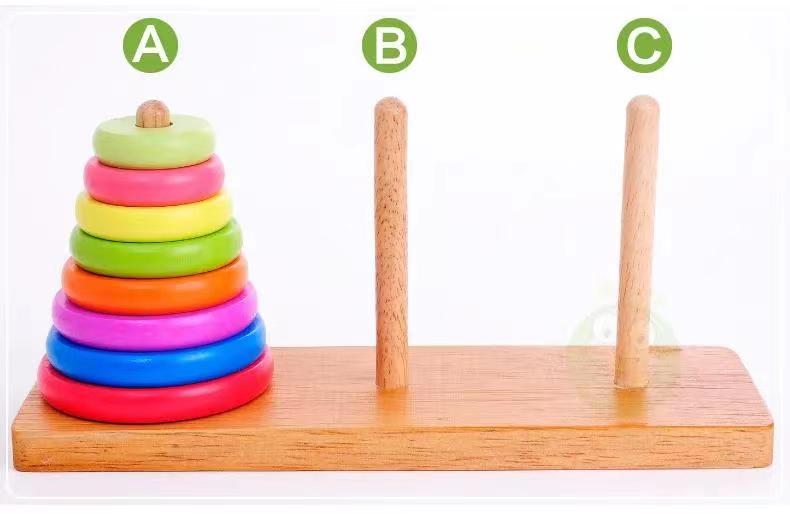
\includegraphics[width=0.8\linewidth]{Hanoi.jpg}
	\caption{ Hanoi塔问题}
\end{figure}
\end{frame}
\begin{frame}
	\sol 记 $f(n)$ 为 $n$ 个圆盘从 $A$ 柱搬到 $C$ 柱所需的最小次数. 整个搬动过程可以人 分成三个阶段:

	(1) 将套在 $A$ 柱上面的 $n-1$ 个圆盘从 $A$ 柱按要求搬到 $B$ 柱,搬动次数为 $f(n-1)$;\\
	(2) 把 $A$ 柱上最下面的那个圆盘搬到 $C$ 柱上,搬动次数为 1 ;\\
	(3) 把 $B$ 柱上的 $n-1$ 个圆盘按要求搬到 $C$ 柱上, 搬动次数为 $f(n-1)$.

	 由加法原则知
	$$
	f(n)=2 f(n-1)+1,
	$$
	又显然 $f(1)=1$, 所以有如下带有初值的递推关系
	$$
	\left\{\begin{array}{l}
	f(n)=2 f(n-1)+1, \\
	f(1)=1 .
	\end{array}\right.
	$$
\end{frame}
\begin{frame}
	\begin{ex}
		在信道上传输由 $a, b, c$ 三个字母组成的长为 $n$ 的字符串, 若字符串中 有两个 $a$ 连续出现, 则信道就不能传输. 令 $f(n)$ 表示信道可以传输的长为 $n$ 的字 符串的个数, 求 $f(n)$ 满足的递推关系.
	\end{ex}
\pause\sol
信道上能够传输的长度为 $n(n \geqslant 2)$ 的字符串可分成如下四类:\\
(1) 最左字符为 $b$;\\
(2) 最左字符为 $c$;\\
(3) 最左两个字符为 $a b$;\\
(4) 最左两个字符为 $a c$.\\
前两类字符串分别有 $f(n-1)$ 个, 后两类字符串分别有 $f(n-2)$ 个. 容易求出 $f(1)=3, f(2)=8$, 从而得到
$$
\left\{\begin{array}{l}
f(n)=2 f(n-1)+2 f(n-2) \quad(n \geqslant 3), \\
f(1)=3, \quad f(2)=8 .
\end{array}\right.
$$
\end{frame}

%\begin{frame}
%	\begin{ex}
%		考虑 0,1 字符串中``010" 子串的相继出现问题.例如, 在 110101010101 中, 我们说``010" 在第 5 位和第 9 位出现, 而不是在第 7 位和第 11 位出现, 在整个字 符串中``010" 共出现两次. 计算 $n$ 位 0,1 字符串中``010" 子串在第 $n$ 位出现的字符 串有多少?
%	\end{ex}
%\pause\sol
%\begin{itemize}
%	\item 设``010" 子串在第 $n$ 位出现的长为 $n$ 的 0,1 字符串的个数为 $f(n)$, 显然 $f(3)=1, f(4)=2, f(5)=3$.
%	\item 最后三位是``010"的$n$位0,1字符串有$2^{n-3}$个
%	\begin{itemize}
%		\item ``010"在第$n$位 出现有$f(n)$个;
%		\item 而 ``010" 不在第 $n$ 位出现, 当且仅当最后 5 位形如``01010",也即``010"在第$n-2$位出现,计数为$f(n-2)$.
%	\end{itemize}
%\end{itemize}
%从而有
%	$$
%\left\{\begin{array}{l}
%	f(n)=2^{n-3}-f(n-2) \quad(n \geqslant 5), \\
%	f(3)=1, \quad f(4)=2.
%\end{array}\right.
%$$
%\end{frame}
%
\begin{frame}
	\begin{ex}
		设$P$是平面上$n$个连通区域$D_{1},\dots,D_{n}$的公共交界点,如图所示。现用$k$种颜色对其着色,要求有公共边界的区域不能有相同的颜色。令$f(n)$表示不同的着色方案数,求它所满足的递推关系。
	\end{ex}
\begin{figure}[h]
	\centering
	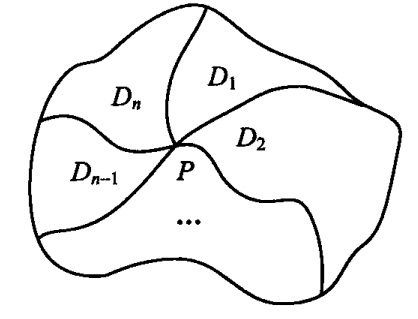
\includegraphics[width=0.5\linewidth]{zone coloring.jpg}
	\caption{ 区域着色}
\end{figure}
\end{frame}
\begin{frame}
	\sol 将所有满足要求的着色方案分成两类 $(n \geqslant 4)$ :

\begin{enumerate}
	\item  $D_1$ 与 $D_{n-1}$ 同色. 此时, $D_n$ 有 $k-1$ 种着色方案. 可将 $D_1$ 与 $D_{n-2}$ 看成相邻 区域, $D_1, D_2, \cdots, D_{n-2}$ 的着色方案数为 $f(n-2)$. 故此类着色方案数为 $(k-1) f(n-2)$.
	\item  $D_1$ 与 $D_{n-1}$ 异色. 此时, $D_n$ 有 $k-2$ 种着色方案. 此时, 可将 $D_1$ 与 $D_{n-1}$ 看 成相邻的区域. 又 $D_1, D_2, \cdots, D_{n-1}$ 用 $k$ 种颜色着色的方案数为 $f(n-1)$, 故此类着 色方案数为 $(k-2) f(n-1)$.
\end{enumerate}
	容易求得 $f(2)=k(k-1), f(3)=k(k-1)(k-2)$, 从而有
	$$
	\left\{\begin{array}{l}
		f(n)=(k-1) f(n-2)+(k-2) f(n-1) \quad(n \geqslant 4), \\
		f(2)=k(k-1), \quad f(3)=k(k-1)(k-2) .
	\end{array}\right.
	$$
\end{frame}

\begin{frame}
	\begin{ex}
		设 $X$ 是一具有乘法运算的代数系统,乘法不满足结合律,用 $x y$ 表示 $x$ 对 $y$ 之积. 如果
		$$
		x_1, x_2, \cdots, x_n \in X,
		$$
		而且这 $n$ 个元素依上面列出的顺序所能作出的一切可能的积彼此不同, 其个数记 为 $f(n)$, 求 $f(n)$ 满足的递推关系.
	\end{ex}
\pause\sol 例如, 对于 $x_1, x_2, x_3 \in X$, 符合题意的积有 2 个:
$$
\left(x_1 x_2\right) x_3, \quad x_1\left(x_2 x_3\right),
$$
所以 $f(3)=2$.

如果在 $x_1 x_2 \cdots x_n$ 的某些字母间加上括号, 但不改变字母间的相互位置关系, 使得这 $n$ 个字母间的乘法可以按所加括号指明的运算方式进行运算,那么 $f(n)$ 就 是加括号的方法的个数.
\end{frame}
\begin{frame}
	\begin{itemize}
		\item 最外层的两对括号形如
		$$
		\left(x_1 \cdots x_r\right)\left(x_{r+1} \cdots x_n\right) \quad(1 \leqslant r \leqslant n-1).
		$$
		\item 当 $r=1$ 或 $n-1$ 时,通常简记为
		$$
		\begin{aligned}
			&x_1\left(x_2 \cdots x_n\right)=\left(x_1\right)\left(x_2 \cdots x_n\right), \\
			&\left(x_1 \cdots x_{n-1}\right) x_n=\left(x_1 \cdots x_{n-1}\right)\left(x_n\right) .
		\end{aligned}
		$$
		\item 在前一个括号中有 $f(r)$ 种加括号的方法, 在后一个括号中又有 $f(n-r)$ 种加括号 的方法, 当 $r$ 遍历 $1,2, \cdots, n-1$ 时, 就得到
		$$
		\begin{aligned}
			f(n)=& f(1) f(n-1)+f(2) f(n-2)+\cdots \\
			&+f(n-2) f(2)+f(n-1) f(1) \\
			=& \sum_{i=1}^{n-1} f(i) f(n-i) \quad(n>1) .
		\end{aligned}
		$$
		\item 初始值为
		$$
		f(1)=1, \quad f(2)=1
		$$
	\end{itemize}
\end{frame}


\begin{frame}
    \begin{ex}
        平面上 $n$ 个圆相互交叠最多可将平面分成多少个区域?
    \end{ex}
    \pause
    \sol 记所求为 $h_n$, 则 $h_1=2$. 显而易见, 将平面分成最多个区域的情形发生在每两个圆都相交 的情形. $n \geqslant 2$ 时, 先把 $n-1$ 个圆在平面上相互交叠, 将平面分成 $h_{n-1}$ 个区域, 再考察将第 $n$ 个圆加入的情形, 可得第 $n$ 个圆与前 $n-1$ 个圆有 $2(n-1)$ 个交点, 这些交点把第 $n$ 个圆 分成 $2(n-1)$ 个圆弧, 每个圆弧把其所在的原有区域分成两个, 即比原来多出 1 个区域, 故共 多出 $2(n-1)$ 个区域, 所以
    $$
    h_n=h_{n-1}+2(n-1) .
    $$
    \pause
    推导下
    去, 当 $n \geq 2$ 时有
    $$
    \begin{aligned}
        h_n &=h_{n-1}+2(n-1) =h_{n-2}+2(n-2)+2(n-1) \\
        &=h_1+2(1)+\cdots+2(n-2)+2(n-1) \\
        &=2+2 \cdot \frac{n(n-1)}{2} \\
        &=n^2-n+2 .
    \end{aligned}
    $$
    上式对 $n=1$ 也成立, 故所求为 $n^2-n+2$.
\end{frame}
\section{常系数线性齐次递推关系的求解}

\begin{frame}
	\begin{defi}[$k$阶线性递推关系]
        \begin{itemize}
\item 设 $k$ 是给定的正整数, 若数列 $f(0), f(1), \cdots, f(n), \cdots$ 的相邻 $k+1$ 项间满足关系
\[
f(n)=c_1(n) f(n-1)+c_2(n) f(n-2)+\cdots+c_k(n) f(n-k)+g(n)\tag{6.2.1}
\]
$n \geqslant k$ 成立, 其中 $c_k(n) \neq 0$, 则称该关系为 $\{f(n)\}$ 的 \blue{$k$ 阶线性递推关系}.

\item 如果 $c_1(n), c_2(n), \cdots, c_k(n)$ 都是常数, 则称之为 $k$ 阶\blue{常系数}线性递推关系.

\item 如果 $g(n)=0$, 则称之为\blue{齐次}的.
        \end{itemize}

	\end{defi}
\begin{itemize}
	\item 如果有一个数列代人递推关系 (6.2.1), 使得其对任何 $n \geqslant k$ 都成立, 则称这 个数列是递推关系 $(6.2 .1)$ 的解.
	\item 常系数线性齐次递推关系的一般形式为
	\[
	f(n)=c_1 f(n-1)+c_2 f(n-2)+\cdots
	+c_k f(n-k) \quad\left(n \geqslant k, c_k \neq 0\right) . \tag{6.2.2}
	\]
\end{itemize}
\end{frame}

\begin{frame}
	\begin{defi}{递推关系特征方程}
        \begin{itemize}
\item 	方程
\[
x^k-c_1 x^{k-1}-c_2 x^{k-2}-\cdots-c_k=0\tag{6.2.3}
\]
叫作递推关系 (6.2.2) 的 \blue{特征方程}.
\item  它的 $k$ 个根 $q_1, q_2, \cdots, q_k$ (可能有重根) 叫作该 递推关系的\blue{特征根}, 其中, $q_i(i=1,2, \cdots, k)$ 是复数.
        \end{itemize}

	\end{defi}
\begin{lem}
	设 $q$ 是非零复数, 则
   \begin{center}
    $f(n)=q^n$ 是递推关系 $(6.2 .2)$ 的解 \,
当且 仅当 \,  $q$ 是它的 \blue{特征根}.
   \end{center}

\end{lem}

\end{frame}

\begin{frame}
	\pf 因为 $h_1(n), h_2(n)$ 都是递推关系 (6.2.2) 的解, 所以
	$$\begin{aligned}
		&b_1 h_1(n)+b_2 h_2(n)\\
		=&b_1\left(c_1 h_1(n-1)+\cdots+c_k h_1(n-k)\right)
		+b_2\left(c_1 h_2(n-1)+\cdots+c_k h_2(n-k)\right) \\
		=& c_1\left(b_1 h_1(n-1)+b_2 h_2(n-1)\right)+\cdots+c_k\left(b_1 h_1(n-k)+b_2 h_2(n-k)\right),
	\end{aligned}
	$$
	从而 $b_1 h_1(n)+b_2 h_2(n)$ 也是递推关系 (6.2.2) 的解.

	由引理 6.2.1 和引理 $6.2 .2$ 知, 若 $q_1, q_2, \cdots, q_k$ 是递推关系 (6.2.2) 的特征 根, $b_1, b_2, \cdots, b_k$ 是常数,那么
	$$
	f(n)=b_1 q_1{ }^n+b_2 q_2{ }^n+\cdots+b_k q_k{ }^n
	$$
	也是递推关系 $(6.2 .2)$ 的解.
\end{frame}
\begin{frame}
	\begin{defi}
		如果对于递推关系 (6.2.2) 的每个解 $h(n)$, 都可以选择一组常 数 $c_1{ }^{\prime}, c_2{ }^{\prime}, \cdots, c_k{ }^{\prime}$, 使得
		$$
		h(n)=c_1{ }^{\prime} q_1{ }^n+c_2{ }^{\prime} q_2{ }^n+\cdots+c_k{ }^{\prime} q_k{ }^n
		$$
		成立, 则称 $b_1 q_1{ }^n+b_2 q_2{ }^n+\cdots+b_k q_k{ }^n$ 是递推关系 (6.2.2) 的通解, 其中, $b_1, b_2$, $\cdots, b_k$ 为任意常数.
	\end{defi}
\begin{thm}
	设 $q_1, q_2, \cdots, q_k$ 是递推关系 (6.2.2) 的 $k$ 个互不相等的特征根, 则
	\[
	f(n)=b_1 q_1{ }^n+b_2 q_2{ }^n+\cdots+b_k q_k{ }^n\tag{6.2.4}
	\]
	是递推关系 (6.2.2) 的通解.
\end{thm}
\pf 由前面的分析可知, 对任意一组 $b_1, b_2, \cdots, b_k, f(n)$ 是递推关系 (6.2.2) 的解.
下面证明: 递推关系 (6.2.2) 的任意一个解 $h(n)$ 都可以表示成 $(6.2 .4)$ 的形 式. $h(n)$ 是 (6.2.2) 的解, 故 $h(n)$ 由 $k$ 个初值 $h(0)=a_0, h(1)=a_1, \cdots$, $h(k-1)=a_{k-1}$ 唯一地确定.
\end{frame}

\begin{frame}
	\pf
	 若 $h(n)$ 可以表示成式(6.2.4) 的形式, 则有
	\[
	\left\{\begin{array}{l}
		b_1+b_2+\cdots+b_k=a_0, \\
		b_1 q_1+b_2 q_2+\cdots+b_k q_k=a_1, \\
		\cdots, \\
		b_1 q_1{ }^{k-1}+b_2 q_2{ }^{k-1}+\cdots+b_k q_k{ }^{k-1}=a_{k-1} .
	\end{array}\right.\tag{6.2.5}
	\]
	如果方程组 (6.2.5) 有唯一解 $b_1{ }^{\prime}, b_2{ }^{\prime}, \cdots, b_k{ }^{\prime}$, 这说明可以找到 $k$ 个常数 $b_1{ }^{\prime}, b_2{ }^{\prime}$, $\cdots, b_k{ }^{\prime}$, 使得
	$$
	h(n)=b_1{ }^{\prime} q_1{ }^n+b_2{ }^{\prime} q_2{ }^n+\cdots+b_k{ }^{\prime} q_k{ }^n
	$$
	成立, 从而 $b_1 q_1{ }^n+b_2 q_2{ }^n+\cdots+b_k q_k{ }^n$ 是该递推关系的通解. 考察方程组 (6.2.5), 它的系数行列式为$$
	\left|\begin{array}{cccc}
		1 & 1 & \cdots & 1 \\
		q_1 & q_2 & \cdots & q_k \\
		\vdots & \vdots & \vdots & \vdots \\
		q_1{ }^{k-1} & q_2{ }^{k-1} & \cdots & q_k{ }^{k-1}
	\end{array}\right|=\prod_{1 \leqslant i<j \leqslant k}\left(q_j-q_i\right)
	$$
	这是著名的 Vandermonde 行列式. 因为 $q_1, q_2, \cdots, q_k$ 互不相等, 所以该行列式不 等于零,这也就是说方程组 (6.2.5) 有唯一解. 所以, $h(n)$ 可以表示成式 (6.2.4) 的形式.
	故式 (6.2.4) 是递推关系 (6.2.2) 的通解.
\end{frame}

\begin{frame}
	\begin{ex}
		求解 6.1 节例 2 中的递推关系
		$$
		\left\{\begin{array}{l}
			f(n)=2 f(n-1)+2 f(n-2), \\
			f(1)=3, \quad f(2)=8 .
		\end{array}\right.
		$$
	\end{ex}
\end{frame}

\begin{frame}
	\sol 先求这个递推关系的通解. 它的特征方程为$$
	x^2-2 x-2=0
	$$
	解这个方程,得
	$$
	x_1=1+\sqrt{3}, \quad x_2=1-\sqrt{3} .
	$$
	所以,通解为

	$f(n)=c_1\left(1+\sqrt{3}\right)^n+c_2 \left (1-\sqrt{3}\right)^n$.
	代入初值来确定$c_{1}$和
	$c_2$ ,得
	$$
	\left\{\begin{array}{l}
		c_1 \left(1+\sqrt{3}\right)+c_2\left(1-\sqrt{3}\right)=3, \\
		c_1\left(1+\sqrt{3}\right)^2+c_2\left(1-\sqrt{3}\right)^2=8 .
	\end{array}\right.
	$$
	求解这个方程组, 得
	$$
	c_1=\frac{2+\sqrt{3}}{2 \sqrt{3}}, \quad c_2=\frac{-2+\sqrt{3}}{2 \sqrt{3}} .
	$$
	因此, 所求的字符串个数为
	$$
	f(n)=\frac{2+\sqrt{3}}{2 \sqrt{3}}\left(1+\sqrt{3}\right)^n+\frac{-2+\sqrt{3}}{2 \sqrt{3}}\left(1-\sqrt{3}\right)^n \quad(n=1,2, \cdots) .
	$$
\end{frame}

%\begin{frame}
%	\begin{ex}
%		核反应堆中有 $\alpha$ 和 $\beta$ 两种粒子,每秒钟内一个 $\alpha$ 粒子可反应产生三个 $\beta$ 粒子,而一个 $\beta$ 粒子又可反应产生一个 $\alpha$ 粒子和两个 $\beta$ 粒子. 若在时刻 $t=0$ 时反应 堆中只有一个 $\alpha$ 粒子, 问 $t=100$ 秒时反应堆中将有多少个 $\alpha$ 粒子?多少个 $\beta$ 粒子? 共有多少个粒子?
%	\end{ex}
%\pause\sol 设在 $t$ 时刻的 $\alpha$ 粒子数为 $f(t), \beta$ 粒子数为 $g(t)$, 根据题设,可以列出下面 的递推关系
%\begin{align}
%	g(t)& =3 f(t-1)+2 g(t-1) \quad(t \geqslant 1) \tag{6.2.6} \\
%	f(t)& =g(t-1) \quad(t \geqslant 1) \tag{6.2.7}
%\end{align}
%以及初值 $g(0) =0, \quad f(0)=1$.
%	由式(6.2.7) 得到
%$$f(t-1)=g(t-2),$$
%把这个等式代入式(6.2.6)得
%$$
%\left\{\begin{array}{l}
%	g(t)=3 g(t-2)+2 g(t-1) \quad(t \geqslant 2), \\
%	g(0)=0, \quad g(1)=3 .
%\end{array}\right.
%$$
%\end{frame}

%%\begin{frame}
%%	递推关系 (6.2.8) 的特征方程为$$
%%	x^2-2 x-3=0,
%%	$$
%%	其特征根为
%%	$$x_{1}=3,\quad x_{2}=-1.$$
%%	所以,该递推关系的通解为
%%	$$
%%	g(t)=c_1 \cdot 3^t+c_2 \cdot(-1)^t .
%%	$$
%%	代人初值 $g(0)=0, g(1)=3$, 得
%%	$$
%%	\left\{\begin{array}{l}
%%		c_1+c_2=0, \\
%%		3 c_1-c_2=3 .
%%	\end{array}\right.
%%	$$
%%	解这个方程组, 得
%%	$$
%%	c_1=\frac{3}{4}, \quad c_2=-\frac{3}{4} .
%%	$$
%%	所以,该递推关系的解为
%%	$$
%%	g(t)=\frac{3}{4} \cdot 3^t-\frac{3}{4} \cdot(-1)^t .
%%	$$
%%\end{frame}
%
%\begin{frame}
%	从而求得
%	$$
%	\begin{aligned}
%		&f(t)=g(t-1)=\frac{3}{4} \cdot 3^{t-1}-\frac{3}{4} \cdot(-1)^{t-1}, \\
%		&f(t)+g(t)=\frac{3}{4} \cdot 3^{t-1}-\frac{3}{4} \cdot(-1)^{t-1}+\frac{3}{4} \cdot 3^t-\frac{3}{4} \cdot(-1)^t=3^t .
%	\end{aligned}
%	$$
%	因此
%	$$
%	\begin{aligned}
%		f(100) &=\frac{3}{4} \cdot 3^{99}-\frac{3}{4} \cdot(-1)^{99} \\
%		&=\frac{3}{4}\left(3^{99}+1\right), \\
%		g(100) &=\frac{3}{4} \cdot 3^{100}-\frac{3}{4} \cdot(-1)^{100}=\frac{3}{4}\left(3^{100}-1\right),
%	\end{aligned}
%	$$故
%	$$
%	f(100)+g(100)=3^{100} .
%	$$
%	\pause
%	\begin{block}{注}
%		对于 $k$ 阶常系数线性齐次递推关系, 当特征根 $q_1, q_2, \cdots, q_k$ 互不相等时, 我们 已经给出了求通解的方法. 但是, 当 $q_1, q_2, \cdots, q_k$ 中有重根时, 这种方法就不再适 用, 换句话说, $c_1 q_1{ }^n+c_2 q_2{ }^n+\cdots+c_k q_k{ }^n$ 就不再是原递推关系的通解. 请看下面 的例子.
%	\end{block}
%\end{frame}

\begin{frame}
	\begin{ex}
		求解递推关系
		$$
		\left\{\begin{array}{l}
			f(n)=4 f(n-1)-4 f(n-2), \\
			f(0)=1, \quad f(1)=3 .
		\end{array}\right.
		$$
	\end{ex}
\pause\sol 递推关系 (6.2.9) 的特征方程为$$
x^2-4 x+4=0,
$$
其特征根为
$$x_1=x_2=2.$$
由引理 6.2.1, 可知 $2^n$ 是递推关系 (6.2.9) 的解(不考虑初值).

\pause
我们不妨试试 $n 2^n$, 把它代人式 (6.2.9), 得
$$
\begin{aligned}
	n 2^n-4(n-1) 2^{n-1}+4(n-2) 2^{n-2} &=n 2^n-(n-1) 2^{n+1}+(n-2) 2^n \\
	&=2^n \left(n-2(n-1)+(n-2) \right) \\
	&=0,
\end{aligned}
$$
这说明 $n 2^n$ 也是递推关系 (6.2.9) 的解.
\end{frame}

\begin{frame}
	易知 $n 2^n$ 与 $2^n$ 线性无关.

     所以原递推关系 的通解为
     $$c_1  2^n+ c_2 n 2^n.$$


	代人初值 $f(0)=1, f(1)=3$, 得
	$$
	\left\{\begin{array}{l}
		c_1=1, \\
		2 c_1+2 c_2=3 .
	\end{array}\right.
	$$

	解这个方程组, 得
	$$
	c_1=1, \quad c_2=\frac{1}{2} .
	$$
	所以,原递推关系的解为
	$$
	f(n)=2^n+2^{n-1} n .
	$$
\end{frame}

%\begin{frame}
%	\textbf{下面分析, 当特征根有重根时, 常系数线性齐次递推关系 (6.2.2) 的通解的一 般形式.}
%
%		设递推关系
%	$$
%	f(n)=c_1 f(n-1)+c_2 f(n-2)+\cdots+c_k f(n-k) \quad\left(n \geqslant k, c_k \neq 0\right)
%	$$的特征方程为
%	$$x^k-c_1 x^{k-1}-c_2 x^{k-2}-\cdots-c_k=0.$$
%	令$$
%	\begin{aligned}
%		P(x) &=x^k-c_1 x^{k-1}-c_2 x^{k-2}-\cdots-c_k, \\
%		P_n(x) &=x^{n-k} \cdot P(x) \\
%		&=x^n-c_1 x^{n-1}-c_2 x^{n-2}-\cdots-c_k x^{n-k} .
%	\end{aligned}
%	$$
%	如果 $q$ 是 $P(x)=0$ 的二重根, 则 $q$ 也是 $P_n(x)=0$ 的二重根, 那么 $q$ 是 $P_n{ }^{\prime}(x)=$ 0 的根. 其中, $P_n{ }^{\prime}(x)$ 是 $P_n(x)$ 的微商, 即
%	$$
%	P_n{ }^{\prime}(x)=n x^{n-1}-c_1(n-1) x^{n-2}-c_2(n-2) x^{n-3}
%	$$
%	因此, $q$ 是 $x P_n^{\prime}(x)=0$ 的根.
%\end{frame}

%\begin{frame}
%	而
%	$$
%	\begin{aligned}
%		x P_n{ }^{\prime}(x)=& n x^n-c_1(n-1) x^{n-1}-c_2(n-2) x^{n-2} \\
%		&-\cdots-c_k(n-k) x^{n-k},
%	\end{aligned}
%	$$
%	代人 $x=q$, 得
%	$$
%	n q^n-c_1(n-1) q^{n-1}-c_2(n-2) q^{n-2}-\cdots-c_k(n-k) q^{n-k}=0 .
%	$$
%	这说明 $n q^n$ 是原递推关系的解.
%	\begin{itemize}
%		\item 类似地可以证明, 如果 $q$ 是 $P(x)=0$ 的三重根, 那么 $q$ 就是 $x P_n{ }^{\prime}(x)=0$ 的二 重根, 即 $q$ 是 $x P_n{ }^{\prime}(x)=0$ 和 $x\left(x P_n{ }^{\prime}(x)\right)^{\prime}=0$ 的根, 从而证明 $n q^n, n^2 q^n$ 也是原 递推关系的解.
%		\item 一般地, 可以证明以下的结论: 如果 $q$ 是 $P(x)=0$ 的 $e$ 重根, 则 $q^n, n q^n$, $n^2 q^n, \cdots, n^{c-1} q^n$ 都是原递推关系的解.
%	\end{itemize}
%
%\end{frame}

\begin{frame}
	\begin{thm}
		设 $q_1, q_2, \cdots, q_{\mathrm{t}}$ 是递推关系 (6.2.2) 的全部不同的特征根, 其重 数分别为 $e_1, e_2, \cdots, e_t\left(e_1+e_2+\cdots+e_t=k\right)$, 那么递推关系 (6.2.2) 的通解为
		$$
		f(n)=f_0(n)+f_1(n)+\cdots+f_t(n),
		$$
		其中
		$$
		f_i(n)=\left(b_{j_1}+b_{j_2} n+\cdots+b_{j_i} n^{e_i-1}\right) \cdot q_i{ }^n \quad(1 \leqslant i \leqslant t) .
		$$
	\end{thm}
%\pf 由前面的讨论知
%$$
%f(n)=f_0(n)+f_1(n)+\cdots+f_t(n)
%$$
%是递推关系 (6.2.2) 的解. 再由初值 $f(0)=a_0, f(1)=a_1, \cdots, f(k-1)=a_k$, 得 到关于 $b_{i j}$ , $1 \leqslant i \leqslant t, 1 \leqslant j \leqslant e_i$ ) 的线性方程组,其系数行列式的值为
%$$
%\prod_{i=1}^t\left(-q_i\right)^{\left(e_i^i\right)} \prod_{1 \leqslant i<j<t}\left(q_j-q_i\right)^{e_i \cdot e_i} \neq 0,
%$$
%故可由初值唯一地确定 $b_i$, 这说明递推关系 (6.2.2) 的任意解均可写成
%$$
%f(n)=\sum_{i=1}^t f_i(n)
%$$
%的形式,其中, $f_i(n)$ 如前所示.
\end{frame}

\begin{frame}
	\begin{ex}
		求解递推关系
		$$
		\left\{\begin{array}{l}
			f(n)=-f(n-1)+3 f(n-2)+5 f(n-3)+2 f(n-4), \\
			f(0)=1, \quad f(1)=0, \quad f(2)=1, \quad f(3)=2 .
		\end{array}\right.
		$$
	\end{ex}
\pause\sol
该递推关系的特征方程为
$$
x^4+x^3-3 x^2-5 x-2=0,
$$
其特征根为
$$
x_1=x_2=x_3=-1, \quad x_4=2 \text {. }
$$
由定理 $6.2 .2$, 对应于 $x=-1$ 的解为
$$
f_0(n)=c_1(-1)^n+c_2 n(-1)^n+c_3 n^2(-1)^n \text {, }
$$
对应于 $x=2$ 的解为
$$
f_2(n)=c_4 2^n .
$$
因此,递推关系的通解为
$$
\begin{aligned}
	f(n) &=f_0(n)+f_2(n) \\
	&=c_1(-1)^n+c_2 n(-1)^n+c_3 n^2(-1)^n+c_4 2^n .
\end{aligned}
$$
\end{frame}

\begin{frame}
	代人初始值,得到方程组
	$$
	\left\{\begin{array}{l}
		c_1+c_4=1, \\
		-c_1-c_2-c_3+2 c_4=0 \\
		c_1+2 c_2+4 c_3+4 c_4=1, \\
		-c_1-3 c_2-9 c_3+8 c_4=2,
	\end{array}\right.
	$$
	解这个方程组,得
	$$
	c_1=\frac{7}{9}, \quad c_2=-\frac{1}{3}, \quad c_3=0, \quad c_4=\frac{2}{9} .
	$$
	所以,原递推关系的解为
	$$
	f(n)=(-1)^n \frac{7}{9}-(-1)^n \frac{1}{3} n+\frac{2}{9} \cdot 2^n .
	$$
\end{frame}

\section{常系数线性非齐次递推关系的求解}
\begin{frame}
	$k$ 阶常系数线性非齐次递推关系的一般形式为
	\[
	f(n)=c_1 f(n-1)+c_2 f(n-2)+\cdots+c_k f(n-k)+g(n) \quad(n \geqslant k),\tag{ 6.3.1 }
	\]
	其中, $c_1, c_2, \cdots, c_k$ 为常数, $c_k \neq 0, g(n) \neq 0$. 递推关系 (6.3.1) 对应的齐次递推 关系为
	\[
	f(n)=c_1 f(n-1)+c_2 f(n-2)+\cdots+c_k f(n-k) . \tag{ 6.3.2 }
	\]
	\begin{thm}
		$k$ 阶常系数线性非齐次递推关系 (6.3.1) 的通解是递推关系 (6.3.1) 的特解加上其相应的齐次递推关系 (6.3.2) 的通解.
	\end{thm}
\end{frame}

\begin{frame}
	\pf
	设 $f_0(n)$ 是递推关系 $(6.3 .1)$ 的特解, $f_2(n)$ 是递推关系 $(6.3 .2)$ 的解,
	则
	$$
	\begin{aligned}
		f_0(n)+f_2(n)=& {\left(c_1 f_0(n-1)+c_2 f_0(n-2)+\cdots\right.} \\
		&\left.+c_k f_0(n-k)+g(n)\right) \\
%		&+\left(c_1 f_2(n-1)+c_2 f_2(n-2)+\cdots+c_k f_2(n-k)\right) \\
		=& c_1\left(f_0(n-1)+f_2(n-1)\right)+\cdots \\
		&+c_k\left(f_0(n-k)+f_2(n-k)\right)+g(n) .
	\end{aligned}
	$$
	所以, $f_0(n)+f_2(n)$ 是递推关系 $(6.3 .1)$ 的解.

	反之, 任给递推关系 (6.3.1) 的一个解 $f(n)$, 与上类似, 可以证明 $f(n)-$ $f_0(n)$ 是递推关系 (6.3.2) 的解. 而 $f(n)=\left(f(n)-f_0(n)\right)+f_0(n)$, 所以 $f(n)$ 可 以表示成 $f_0(n)$ 与递推关系 $(6.3 .2)$ 的解之和.

	综合以上分析, 定理成立.
\end{frame}

\begin{frame}
	对于一般的 $g(n), k$ 阶常系数线性非齐次递推关系 (6.3.1) 没有普遍的解法, 只有在某些简单的情况下, 可以用待定系数法求出递推关系 (6.3.1) 的特解. 表 6.3.1 对于几种 $g(n)$ 给出了递推关系 (6.3.1) 的特解 $f_0(n)$ 的一般形式. 在 $6.5$ 节, 我们将用生成函数的方法证明表 6.3.1 中特解的正确性.
\begin{table}[h]

		\caption{6.3.1}
			\vspace{-2.0em}
	\begin{tabular}{c||c|c}
		\hline$g(n)$ & 特征多项式 $P(x)$ & 特解 $f_0(n)$ 的一般形式 \\
		\hline \hline $\beta^n$ & $P(\beta) \neq 0$ & $a \beta^n$ \\
		\cline { 2 - 3 } & $\beta$ 是 $P(x)=0$ 的 $m$ 重根 & $a n^m \beta^n$ \\
		\hline {$n^s$} & $P(1) \neq 0$ & $b_s n^s+b_{s-1} n^{s-1}+\cdots+b_1 n+b_0$ \\
		\cline { 2 - 3 } & 1 是 $P(x)=0$ 的 $m$ 重根 & $n^m\left(b_s n^s+b_{s-1} n^{s-1}+\cdots+b_1 n+b_0\right)$ \\
		\hline {$n^s \beta^n$} & $P(\beta) \neq 0$ & $\left(b_s n^s+b_{s-1} n^{s-1}+\cdots+b_1 n+b_0\right) \beta^n$ \\
		\cline { 2 - 3 } & $\beta$ 是 $P(x)=0$ 的 $m$ 重根 & $n^m\left(b_s n^s+b_{s-1} n^{s-1}+\cdots+b_1 n+b_0\right) \beta^n$ \\
		\hline
	\end{tabular}
\end{table}
\end{frame}

\begin{frame}
	\begin{ex}
		求解递推关系
		$$
		\left\{\begin{array}{l}
			f(n)=2 f(n-1)+4^{n-1}, \\
			f(0)=1 .
		\end{array}\right.
		$$
	\end{ex}
\pause\sol
因为 4 不是特征方程的根, 所以该递推关系的非齐次特解为 $4^{n-1} a$. 将其 代人递推关系, 得
比较等式两边 $4^{n-1}$ 的系数, 得
$$
a=\frac{1}{2} a+1,
$$
从而
而相应齐次递推关系的通解为 $2^n c$, 由定理 6.3.1 知, 非齐次递推关系的通解为 由初值 $f(0)=1$, 得
$$
f(n)=2^n c+4^{n-1} \cdot 2 .
$$
$$
2^0 c+4^{0-1} \cdot 2=1,
$$
从而
$$
c=\frac{1}{2},
$$
故
$$
f(n)=\frac{1}{2}\left(2^n+4^n\right) .
$$
\end{frame}

%\begin{frame}
%	\begin{block}{注}
%		从例 1 可以看出, 求解常系数线性非齐次递推关系的基本步骤是: 首先用待定 系数法通过递推关系 (不带初值) 求出特解, 然后用常系数线性齐次递推关系的通 解与初值解出递推关系的解.
%	\end{block}
%\pause\begin{ex}
%	求和 $1^4+2^4+\cdots+n^4$.
%\end{ex}
%\pause\sol
%令
%$$
%f(n)=1^4+2^4+\cdots+n^4,
%$$
%它满足递推关系
%$$
%\left\{\begin{array}{l}
%	f(n)=f(n-1)+n^4, \\
%	f(0)=0 .
%\end{array}\right.
%$$
%因为 1 是特征方程的一重根, 所以该递推关系的特解为
%$$
%n\left(b_4 n^4+b_3 n^3+b_2 n^2+b_1 n+b_0\right) \text {. }
%$$
%\end{frame}
%
%\begin{frame}
%	将其代人递推关系, 并比较等号两边 $n^i(0 \leqslant i \leqslant 4)$ 的系数, 得到
%	$$
%	\left\{\begin{array}{l}
%		-5 b_4+b_3+1=b_3, \\
%		10 b_4-4 b_3+b_2=b_2, \\
%		-10 b_4+6 b_3-3 b_2+b_1=b_1, \\
%		5 b_4-4 b_3+3 b_2+2 b_1+b_0=b_0, \\
%		-b_4+b_3-b_2+b_1-b_0=0 .
%	\end{array}\right.
%	$$
%	解得
%	$$
%	b_0=\frac{1}{30}, b_1=0, b_2=\frac{1}{3}, b_3=\frac{1}{2}, b_4=\frac{1}{5},
%	$$
%	即非齐次特解为
%	$$
%	f_0(n)=\frac{n}{30}\left(6 n^4+15 n^3+10 n^2-1\right) .
%	$$
%	而相应齐次递推关系的通解为
%	$$f_2(n)=1^{n}c.$$
%
%	由定理 6.3.1 知, 非齐次通解为
%	$$
%	\begin{aligned}
%		f(n) &=f_0(n)+f_2(n) \\
%		&=c+\frac{n}{30}\left(6 n^4+15 n^3+10 n^2-1\right) .
%	\end{aligned}
%	$$
%\end{frame}
%
%\begin{frame}
%	又由 $f(0)=0$ 可求得 $c=0$, 故
%	$$
%	\begin{aligned}
%		f(n) &=\frac{n}{30}\left(6 n^4+15 n^3+10 n^2-1\right) \\
%		&=\frac{n}{30}(n+1)(2 n+1)\left(3 n^2+3 n-1\right) .
%	\end{aligned}
%	$$
%\end{frame}

\begin{frame}
	\begin{ex}
		求解递推关系
		$$
		\left\{\begin{array}{l}
			f(n)-4 f(n-1)+4 f(n-2)=n \cdot 2^n, \\
			f(0)=0, \quad f(1)=1 .
		\end{array}\right.
		$$
	\end{ex}
\pause\sol
 由于 2 是特征方程的二重根, 所以该递推关系的特解为
$$
f_0(n)=n^2\left(b_1 n+b_0\right) \cdot 2^n .
$$
将它代人递推关系, 并比较等号两边 $n$ 的系数及常数项,得到
$$
\left\{\begin{array}{l}
	6 b_1=1, \\
	-6 b_1+2 b_0=0,
\end{array}\right.
$$
解得
$$
b_0=\frac{1}{2}, \quad b_1=\frac{1}{6} .
$$
而相应齐次递推关系的通解为 $\left(c_0+c_1 n\right) \cdot 2^n$, 从而非齐次递推关系的通解为
$$
f(n)=\left( \left(c_0+c_1 n\right)+n^2\left(\frac{n}{6}+\frac{1}{2}\right) \right) \cdot 2^n .
$$

再由初值 $f(0)=0, f(1)=1$, 求得 $c_0=0, c_1=-\frac{1}{6}$.于是
$$
f(n)=\frac{1}{6}\left(n^3+3 n^2-n\right) \cdot 2^n .
$$
\end{frame}

\begin{frame}
	\begin{ex}
		求解 Hanoi 塔问题满足的递推关系
		$$
		\left\{\begin{array}{l}
			f(n)=2 f(n-1)+1, \\
			f(0)=0 .
		\end{array}\right.
		$$
	\end{ex}
\pause\sol
相应的特征方程为 $x=2$, 故齐次通解为 $2^n c$. 设非齐次特解为 $b$, 代人原 递推关系, 得
$$
b-2 b=1 \text {, }
$$
所以特解为 $b=-1$. 根据前面的分析, 可知该递推关系的通解为
$$f(n)=2^n c-1.$$
代入初值$f(0)=0$,得$c=1$.所以
$$
f(n)=2^n-1 .
$$
\end{frame}

\begin{frame}
\begin{ex}
求解非齐次线性递推关系
$$
h_n=6 h_{n-1}-9 h_{n-2}+2 n,(n \geq 2),
$$
初始条件为 $h_0=1, h_1=0$.
\end{ex}
\pause
\sol  先求原递推关系对应的齐次线性递推关系
$$
A_n=6 A_{n-1}-9 A_{n-2}
$$
的通解, 得到 $A_n=(a n+b) 3^n$.


再寻找原非齐次线性递推关系的一个特解. 观察原递推关系特点, 猜想 $B_n=c n+d$ (其 中 $c, d$ 待定) 应为一个特解. 代入原递推关系, 解得 $c=\frac{1}{2}, d=\frac{3}{2}$, 即 $B_n=\frac{1}{2} n+\frac{3}{2}$ 为一个特 解. 故原非齐次线性递推关系的通解可设为
$$
h_n=A_n+B_n=(a n+b) 3^n+\frac{1}{2} n+\frac{3}{2} .
$$
代入初始条件, 解得 $a=-\frac{1}{6}, b=-\frac{1}{2}$. 从而
$$
h_n=\left(-\frac{n}{6}-\frac{1}{2}\right) 3^n+\frac{1}{2} n+\frac{3}{2} .
$$

\end{frame}

\begin{frame}
    \begin{block}{例}
        求解非齐次线性递推关系
        $$
        h_n=6 h_{n-1}-9 h_{n-2}+2 n,(n \geq 2),
        $$
        初始条件为 $h_0=1, h_1=0$.
    \end{block}

    注意, 必须在有了齐次线性递推关系的通解以及非齐次线性递推关系的特解并 将它们相加得到 $A_n+B_n$ 以后, 才可以代入初始条件以获得通解的特征根系数. 这是因为初 始条件是针对满足相应非齐次线性递推关系的数列本身, 而并非其齐次部分.
\end{frame}

\section{用迭代归纳法求解递推关系}

\begin{frame}
\begin{ex}
平面上有 $n$ 条直线, 任意两条直线都不平行, 任意三条直线都不共点, 则这 $n$ 条直线把平面分成多少个部分?
\end{ex}
\pause
\sol
设 $a_n$ 为所求. 易见 $a_0=1, a_1=2, a_2=4, \ldots$

考察第 $n$ 条直线, 在其它直线将平面划分 为 $a_{n-1}$ 个部分的基础上, 第 $n$ 条直线与其它 $n-1$ 条直线有 $n-1$ 个交点, 从而自身被分成 $n$ 段. 每段都将原来 $a_{n-1}$ 块区域中的某部分一分为二, 从而形成 $n$ 块新区域.

故当 $n \geq 1$ 时, $a_n=a_{n-1}+n$.

从而, $a_n=1+1 +2+\cdots+n=1+ \frac{n^2+n}{2}=\frac{n^2+n+2}{2}$.
\end{frame}
%\begin{frame}
%	迭代归纳法也是求解递推关系的一种方法, 尤其对于某些非线性的递推关系, 不存在求解的一般性方法和公式, 不妨用这种方法来试一试. 下面通过几个例子来 说明.
%	\pause
%	\begin{ex}
%		求解递推关系
%		$$
%		\left\{\begin{array}{l}
%			f(n)=f(n-1)+n^3, \\
%			f(0)=0 .
%		\end{array}\right.
%		$$
%	\end{ex}
%\pause\sol
%先用迭代法求解该递推关系, 得
%$$
%\begin{aligned}
%	f(n) &=f(n-1)+n^3 \\
%	&=f(n-2)+(n-1)^3+n^3 \\
%	&=\cdots \\
%	&=f(1)+2^3+\cdots+(n-1)^3+n^3 \\
%	&=f(0)+1^3+2^3+\cdots+(n-1)^3+n^3 \\
%	&=1^3+2^3+\cdots+(n-1)^3+n^3 .
%\end{aligned}
%$$
%\end{frame}
%
%\begin{frame}
%	能否找到 $f(n)$ 的一个简单表达式呢?为此,我们考察该数列的前 5 项,得$$
%	\begin{aligned}
%		f(0) &=0=0^2 \\
%		f(1) &=1^3=1=1^2 \\
%		f(2) &=1^3+2^3=9=3^2 =(1+2)^2, \\
%		f(3) &=1^3+2^3+3^3=36=6^2 =(1+2+3)^2 \\
%		f(4) &=1^3+2^3+3^3+4^3=100=10^2 =(1+2+3+4)^2
%	\end{aligned}
%	$$
%	由此,我们得出 $f(n)$ 的前 5 项满足
%	$$
%	\begin{aligned}
%		f(n) &=(0+1+\cdots+n)^2 \\
%		&=\frac{n^2(n+1)^2}{4} .
%	\end{aligned}
%	$$
%	要证明上式的确是原递推关系的解,我们用归纳法.
%\end{frame}
%
%\begin{frame}
%	当 $n=0$ 时, $f(0)=0$,上式成立.
%	假设 $n=k$ 时上式成立, 即
%	$$
%	f(k)=\frac{1}{4} k^2(k+1)^2,
%	$$
%	则由递推关系, 有
%	$$
%	\begin{aligned}
%		f(k+1) &=f(k)+(k+1)^3 \\
%		&=\frac{1}{4} k^2(k+1)^2+(k+1)^3 \\
%		&=\frac{1}{4}(k+1)^2(k+2)^2 .
%	\end{aligned}
%	$$
%	故由归纳法知
%	$$
%	f(n)=\frac{1}{4} n^2(n+1)^2
%	$$
%	是原递推关系的解.
%	\begin{block}{注}
%		迭代法并不仅仅局限于如例 1 所示的直接导出 $f(n)$ 的表达式. 利用迭代法, 还可以先将原递推关系化简, 然后再求解.
%		下面介绍解递推关系常用的几个技巧.
%	\end{block}
%\end{frame}

\begin{frame}{将非齐次递推关系齐次化}
	\begin{ex}
		求解递推关系
		$$
		\left\{\begin{array}{l}
			f(n)=2 f(n-1)+4^{n-1} \\
			f(1)=3
		\end{array}\right.
		$$
	\end{ex}
\pause\sol
由递推关系 (6.4.1) 可以得到
$$
f(n-1)=2 f(n-2)+4^{n-2},
$$
将上式乘以 $-4$ 后再与式 (6.4.1) 相加, 得
\[
f(n)=6 f(n-1)-8 f(n-2)\tag{6.4.2} .
\]
如此我们得到了二阶齐次递推关系 (6.4.2), 它需要两个初值才能确定解.
\end{frame}

\begin{frame}
	 将 $f(1)$ $=3$ 代人递推关系 (6.4.1), 得
	所以有
	$$
	f(2)=2 f(1)+4^{2-1}=10 \text {. }
	$$
	$$
	\left\{\begin{array}{l}
		f(n)=6 f(n-1)-8 f(n-2), \\
		f(1)=3, \quad f(2)=10 .
	\end{array}\right.
	$$
	它的特征方程为
	$$
	x^2-6 x+8=0,
	$$
	解得两个特征根为
	于是, 通解为
	$$
	x_1=2, \quad x_2=4,
	$$
	$$
	f(n)=A \cdot 2^n+B \cdot 4^n .
	$$
	由初值 $f(1)=3, f(2)=10$, 求得 $A=B=\frac{1}{2}$. 故
	$$
	f(n)=\frac{1}{2}\left(2^n+4^n\right) .
	$$
\end{frame}
%
%\begin{frame}{2. 将变系数的一阶线性递推关系化为常系数线性递推关系}
%	\begin{ex}
%		求解递推关系
%		$$
%		\left\{\begin{array}{l}
%			f(n)=\frac{n+1}{2 n} f(n-1)+1, \\
%			f(0)=1 .
%		\end{array}\right.
%		$$
%	\end{ex}
%\pause\sol
%令
%$$
%\begin{aligned}
%	f(n) &=\frac{n+1}{2 n} \cdot \frac{n}{2(n-1)} \cdot \cdots \cdot \frac{2}{2 \cdot 1} \cdot h(n) \\
%	&=\frac{n+1}{2^n} h(n),
%\end{aligned}
%$$
%代人上述递推关系并化简, 即得到关于 $h(n)$ 的递推关系
%$$
%\left\{\begin{array}{l}
%	h(n)=h(n-1)+\frac{2^n}{n+1}, \\
%	h(0)=1 .
%\end{array}\right.
%$$
%\end{frame}
%\begin{frame}
%	解得
%	$$
%	h(n)=\sum_{k=0}^n \frac{2^k}{k+1},
%	$$
%	$$
%	f(n)=\frac{n+1}{2^n} \sum_{k=0}^n \frac{2^k}{k+1} .
%	$$
%	一般地,一阶线性递推关系可以表示成
%	$$
%	f(n)=c(n) f(n-1)+g(n) .
%	$$
%	令
%	$$
%	\begin{aligned}
%		&f(n)=c(n) c(n-1) \cdots c(1) h(n), \\
%		&(n)=h(n-1)+\frac{g(n)}{c(n) c(n-1) \cdots c(1)},
%	\end{aligned}
%	$$
%	它把变系数化为常系数.
%\end{frame}
%
%\begin{frame}{3.变量代换 化一阶高次递推关系为一阶线性递推关系}
%	\begin{ex}
%		求解递推关系
%		\[
%		\left\{\begin{array}{l}
%			f(n)=3 f^2(n-1), \\
%			f(0)=1 .
%		\end{array}\right.\tag{6.4.3}
%		\]
%	\end{ex}
%\pause\sol
%对递推关系 (6.4.3) 两边取自然对数, 得
%$$
%\ln f(n)=\ln 3+2 \ln f(n-1) .
%$$
%令 $h(n)=\ln f(n)$, 得
%$$
%\left\{\begin{array}{l}
%	h(n)=2 h(n-1)+\ln 3, \\
%	h(0)=0
%\end{array}\right.
%$$
%解得
%$$
%h(n)=\left(2^n-1\right) \ln 3,
%$$
%从而
%$$
%f(n)=3^{2^n-1}
%$$
%\end{frame}

\section{用生成函数求解递推关系}
\begin{frame}
	利用生成函数求解各类递推关系有广泛的适用性,给定关于$f(n)$的递推关系式,求解$f(n)$的基本步骤是:
		\begin{block}{基本步骤}
		\begin{enumerate}
			\item 令$A(x)=\sum_{n=0}^{\infty}f(n)x^{n}$;
			\item 将关于$f(n)$的递推关系式转化成关于$A(x)$的方程式;
			\item 解出$A(x)$,将$A(x)$展开成$x$的幂级数,$x^{n}$的系数即为$f(n)$.
		\end{enumerate}

	\end{block}
\end{frame}

\begin{frame}
\begin{ex}
			求解递推关系
			\[
			\left\{\begin{array}{l}
				f(n)=7f(n-1)-12f(n-2), \\
				f(0)=2,\quad f(1)=7 .
			\end{array}\right.\tag{6.4.3}
			\]
		\end{ex}
		\pause\sol
令$$A(x)=\sum_{n=0}^{\infty}f(n)x^{n},$$ 则有$$
\begin{aligned}
	A(x)-f(0)-f(1) x &=\sum_{n=2}^{\infty} f(n) x^n \\
	&=\sum_{n=2}^{\infty} \left( 7 f(n-1)-12 f(n-2) \right)  x^n \\
	&=7 x \sum_{n=1}^{\infty} f(n) x^n-12 x^2 \sum_{n=0}^{\infty} f(n) x^n \\
	&=7 x \left( A(x)-f(0) \right) -12 x^2 A(x)
\end{aligned}
$$
\end{frame}

\begin{frame}
	将 $f(0)=2, f(1)=7$ 代人上式并整理, 得
	$$
	A(x)=\frac{2-7 x}{1-7 x+12 x^2}=\frac{1}{1-3 x}+\frac{1}{1-4 x}=\sum_{n=0}^{\infty}\left(3^n+4^n\right) x^n \text {, }
	$$
	所以
	$$
	f(n)=3^n+4^n
	$$
\end{frame}

\begin{frame}
	\begin{ex}
		求解递推关系$$
		\left\{\begin{array}{l}
			f(n)=4 f(n-1)-4 f(n-2) \quad(n \geqslant 2) \\
			f(0)=0, \quad f(1)=1 .
		\end{array}\right.
		$$
	\end{ex}
\pause\sol
令
$$
A(x)=\sum_{n=0}^{\infty} f(n) x^n,
$$
则有
$$
\begin{aligned}
	A(x)-f(0)-f(1) x &=\sum_{n=2}^{\infty} f(n) x^n \\
	&=\sum_{n=2}^{\infty}[4 f(n-1)-4 f(n-2)] x^n \\
	&=4 x \sum_{n=1}^{\infty} f(n) x^n-4 x^2 \sum_{n=0}^{\infty} f(x) x^n \\
	&=4 x \cdot[A(x)-f(0)]-4 x^2 A(x) .
\end{aligned}
$$
\end{frame}

\begin{frame}
	将 $f(0)=0, f(1)=1$ 代人上式并整理, 得
	$$
	A(x)=\frac{x}{4 x^2-4 x+1}=\frac{x}{(1-2 x)^2} .
	$$
	设
	$$
	A(x)=\frac{C_1}{1-2 x}+\frac{C_2}{(1-2 x)^2},
	$$
	其中, $C_1, C_2$ 为待定系数. 通过比较等式两边分子的常数项与 1 次项系数, 可得
	$$
	\left\{\begin{array}{l}
		C_1+C_2=0, \\
		-2 \cdot C_1=1,
	\end{array}\right.
	$$
	所以, $C_1=-\frac{1}{2}, C_2=\frac{1}{2}$.
	$$
	\begin{aligned}
		A(x) &=-\frac{1}{2} \cdot \frac{1}{1-2 x}+\frac{1}{2} \cdot \frac{1}{(1-2 x)^2} \\
		&=-\frac{1}{2} \sum_{n=0}^{\infty} 2^n x^n+\frac{1}{2} \sum_{n=0}^{\infty}\left(\begin{array}{c}
			n+1 \\
			n
		\end{array}\right) \cdot 2^n \cdot x^n .
	\end{aligned}
	$$
	故
	$$
	f(n)=-\frac{1}{2} \cdot 2^n+\frac{1}{2} \cdot(n+1) \cdot 2^n=\frac{1}{2} \cdot n \cdot 2^n=n\cdot 2^{n-1} .
	$$

\end{frame}

\begin{frame}
	\begin{ex}
		求解递推关系
		$$
		\left\{\begin{array}{l}
			f(n)=f(n-1)+n^4, \\
			f(0)=0 .
		\end{array}\right.
		$$
	\end{ex}
\pause\sol
令
$$
A(x)=\sum_{n=0}^{\infty} f(n) x^n,
$$
代人递推关系, 得
\[\begin{aligned}
	A(x)-f(0)=&\sum_{n=1}^{\infty}[f(n-1)+n^{4}]x^{n}\\
	=&x A(x)+\sum_{n=1}^{\infty} n^4 x^n,
\end{aligned}
\]
解得
$$
A(x)=\frac{1}{1-x} \sum_{n=1}^{\infty} n^4 x^n .
$$

\end{frame}

\begin{frame}
	利用
	$$
	G\left\{k^3\right\}=\frac{x\left(1+4 x+x^2\right)}{(1-x)^4},
	$$
	求得
	$$
	G\left\{k^4\right\}=\frac{x\left(1+11 x+11 x^2+x^3\right)}{(1-x)^5}.
	$$
	所以$$
	\begin{aligned}
		A(x) &=\frac{x\left(1+11 x+11 x^2+x^3\right)}{(1-x)^6} \\
		&=\left(x+11 x^2+11 x^3+x^4\right) \sum_{i=1}^{\infty}\binom{i+5}{i} x^i .
	\end{aligned}
	$$
	于是, $x^n$ 的系数 $f(n)$ 为
	$$
	\begin{aligned}
		f(n) &=
		\binom{n-1+5}{n-1}
		+11\binom{n-2+5}{n-2}+11\binom{n-3+5}{n-3}+\binom{n-4+5}{n-4} \\
		&=\frac{1}{30} n(n+1)\left(6 n^3+9 n^2+n-1\right) .
	\end{aligned}
	$$
\end{frame}

\begin{frame}
	\begin{ex}
		求解递推关系
		$$
		\left\{\begin{array}{l}
			f(n)=2 f(n-1)+4^{n-1} \quad(n \geqslant 2), \\
			f(1)=3 .
		\end{array}\right.
		$$
	\end{ex}
\pause\sol
令
$$
A(x)=\sum_{n=1}^{\infty} f(n) x^n,
$$
代人递推关系, 得
$$
\begin{aligned}
	A(x)-f(1) x &=\sum_{n=2}^{\infty}\left( 2 f(n-1)+4^{n-1}\right)  x^n \\
	&=2 x A(x)+4 x^2 \sum_{n=0}^{\infty}(4 x)^n,
\end{aligned}
$$
解得
$$
A(x)=\frac{(3-8 x) x}{(1-2 x)(1-4 x)}=x\left(\frac{1}{1-2 x}+\frac{2}{1-4 x}\right) .
$$
所以, $x^n$ 的系数 $f(n)$ 为
$$
f(n)=\frac{1}{2}\left(2^n+4^n\right) .
$$
\end{frame}

\begin{frame}
	\begin{ex}
		用硬币垒成一个 “喷泉” 如下, 每行的硬币都连续摆在一起, 除最下一行外, 每 枚硬币恰好置于其下面一行的两枚硬币之间. 令 $f(n)$ 表示如此可能㕕成的最下一行恰有 $n$ 枚硬币的 “喷泉” 数. 试求 $\{f(n)\}_{n=0}^{\infty}$ 的普通生成函数.
	\end{ex}
\pause\sol
首先 $f(0)=1$. 对 $n \geq 1$, 若只有一行, 则数目为 1 , 若有多于一行, 设从下面数第二行有 $k$ 枚硬币, 则 $1 \leq k \leq n-1$, 且这 $k$ 枚硬币所在的位置有 $n-k$ 种, 所以
$$
f(n)=\sum_{k=1}^{n-1}(n-k) f(k)+1=\sum_{k=1}^n(n-k) f(k)+1 .
$$
令 $\{f(n)\}_{n=0}^{\infty}$ 的普通生成函数为 $f(x)$. 则
$$
\begin{aligned}
	f(x)=\sum_{n=0}^{\infty} f(n) x^n &=\sum_{n \geq 0}\left(\sum_{k=1}^n(n-k) f(k)+1\right) x^n \\
	&=\sum_{n \geq 0}\left(\sum_{k=1}^n(n-k) f(k)\right) x^n+\sum_{n \geq 0} 1 \cdot x^n \\
	&=\sum_{n \geq 0}\left(\sum_{k=1}^n(n-k) f(k)\right) x^n+\frac{1}{1-x} .
\end{aligned}
$$

\end{frame}

\begin{frame}
	设 $g(x)=f(x)-1$, 即 $g(x)$ 为 $g(n)$ 的普通生成函数, 其中 $g(0)=f(0)-1=0$, 而 $n \geq 1$ 时, $g(n)=f(n)$. 则有
	$$
	\sum_{k=1}^n(n-k) f(k)=\sum_{k=1}^n(n-k) g(k)=\sum_{k=0}^n(n-k) g(k) .
	$$
	然而 $\{n\}_0^{\infty}$ 的普通生成函数是 $(x D) \frac{1}{1-x}=\frac{x}{(1-x)^2}$, 所以
	$$
	\sum_{n=0}^{\infty}\left(\sum_{k=0}^n(n-k) g(k)\right) x^n=\frac{x}{(1-x)^2} g(x)=\frac{x}{(1-x)^2}(f(x)-1) .
	$$
	由
	$$
	f(x)=\frac{x}{(1-x)^2}(f(x)-1)+\frac{1}{1-x},
	$$
	解得
	$$
	f(x)=\frac{1-2 x}{1-3 x+x^2}.
	$$
经过计算, 可求得 $f(n)$ 为
$$
f(n)=\frac{-1+\sqrt{5}}{2 \sqrt{5}}\left(\frac{3+\sqrt{5}}{2}\right)^n+\frac{1+\sqrt{5}}{2 \sqrt{5}}\left(\frac{3-\sqrt{5}}{2}\right)^n .
$$
\end{frame}

\end{document}